%**************************************************************************************
% License:
% CC BY-NC-SA 4.0 (http://creativecommons.org/licenses/by-nc-sa/4.0/)
%**************************************************************************************

\documentclass[notes]{beamer}

\mode<presentation> {

\usetheme{Madrid}

% Burnt orange
\definecolor{burntorange}{rgb}{0.8, 0.33, 0.0}
\colorlet{beamer@blendedblue}{burntorange}
% Pale yellow
\definecolor{paleyellow}{rgb}{1.0, 1.0, 0.953}
\setbeamercolor{background canvas}{bg=paleyellow}
% Secondary and tertiary palett
\setbeamercolor*{palette secondary}{use=structure,fg=white,bg=burntorange!80!black}
\setbeamercolor*{palette tertiary}{use=structure,fg=white,bg=burntorange!60!black}

% To remove the footer line in all slides uncomment this line
%\setbeamertemplate{footline}
% To replace the footer line in all slides with a simple slide count uncomment this line
%\setbeamertemplate{footline}[page number]

% To remove the navigation symbols from the bottom of all slides uncomment this line
%\setbeamertemplate{navigation symbols}{}
}

\usepackage{amsmath}
\usepackage{bm}
\usepackage{breqn}
\usepackage{cancel}
\usepackage{graphicx} % for figures
\usepackage{subcaption} % for subplots 
\usepackage[labelsep=space,tableposition=top]{caption}
\renewcommand{\figurename}{Fig.} 
\usepackage{cleveref}
\usepackage{caption,subcaption}% http://ctan.org/pkg/{caption,subcaption}
\usepackage{booktabs} % Allows the use of \toprule, \midrule and \bottomrule in tables
\usepackage{multirow}
\usepackage{tabularx}
\usepackage{siunitx}
\usepackage{cleveref}

% To print 2 slides on a page
%\usepackage{handoutWithNotes}
%\pgfpagesuselayout{2 on 1}[border shrink=2mm]
%----------------------------------------------------------------------------------------
%	TITLE PAGE
%----------------------------------------------------------------------------------------
% The short title appears at the bottom of every slide, the full title is only on the title page
\title[CE394M: Friction]{CE394M: Friction} 
\author{Krishna Kumar} % name
\institute[UT Austin] % institution 
{
University of Texas at Austin \\
\medskip
\textit{
  \url{krishnak@utexas.edu}} % Your email address
}
\date{} % Date, can be changed to a custom date

\begin{document}

\begin{frame}
\titlepage % title page as the first slide
\end{frame}

\AtBeginSection[]
{
	\begin{frame}<beamer>
		\frametitle{Overview}
		\tableofcontents[currentsection]
	\end{frame}
}

%----------------------------------------------------------------------------------------
\begin{frame}
	\frametitle{Triaxial compression undrained: loose v dense}
	\mode<beamer>{	
		\begin{figure}
			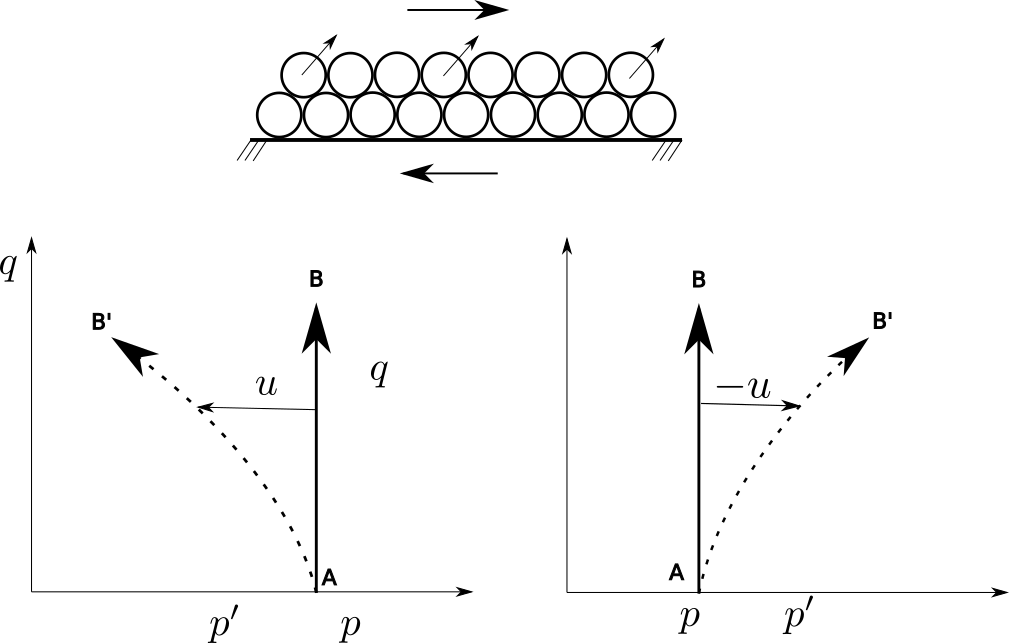
\includegraphics[width=0.85\textwidth]{figs/tx-undrained-pwp.png}
			\caption*{Total and effective stress paths for undrained triaxial test: (a) on soil that wishes to contract as it is sheared, and (b) on soil that wishes to expand as it is sheared.}
		\end{figure}
	}
	\mode<handout>{
		\vspace{6cm}
	}
\end{frame}


%----------------------------------------------------------------------------------------
\begin{frame}
	\frametitle{Friction: Is this correct?}
	\begin{figure}
		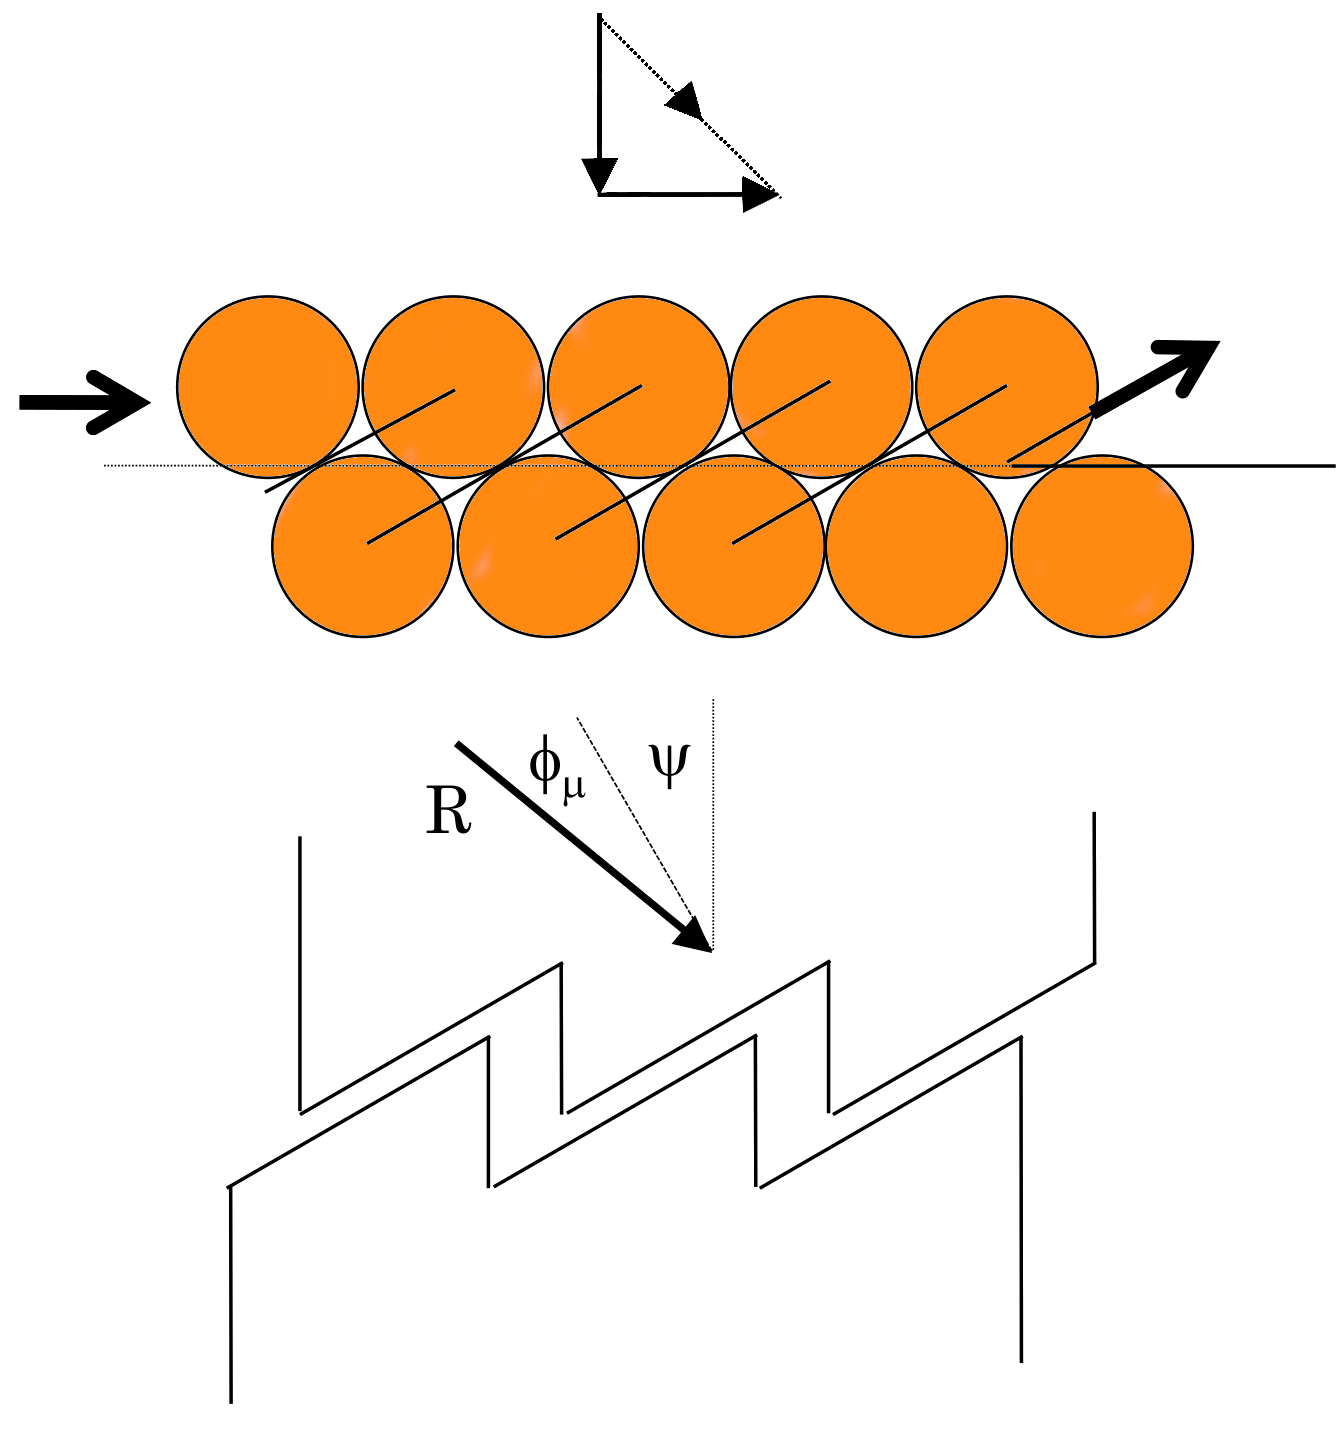
\includegraphics[width=0.5\textwidth]{figs/friction-sawblade.png}
		\caption*{$\phi_{ss} = \phi_\mu + \psi_{ss}$}
	\end{figure}
\end{frame}


%----------------------------------------------------------------------------------------
\begin{frame}
	\frametitle{Macroscopically, as soil aggregates...}
	\begin{figure}
		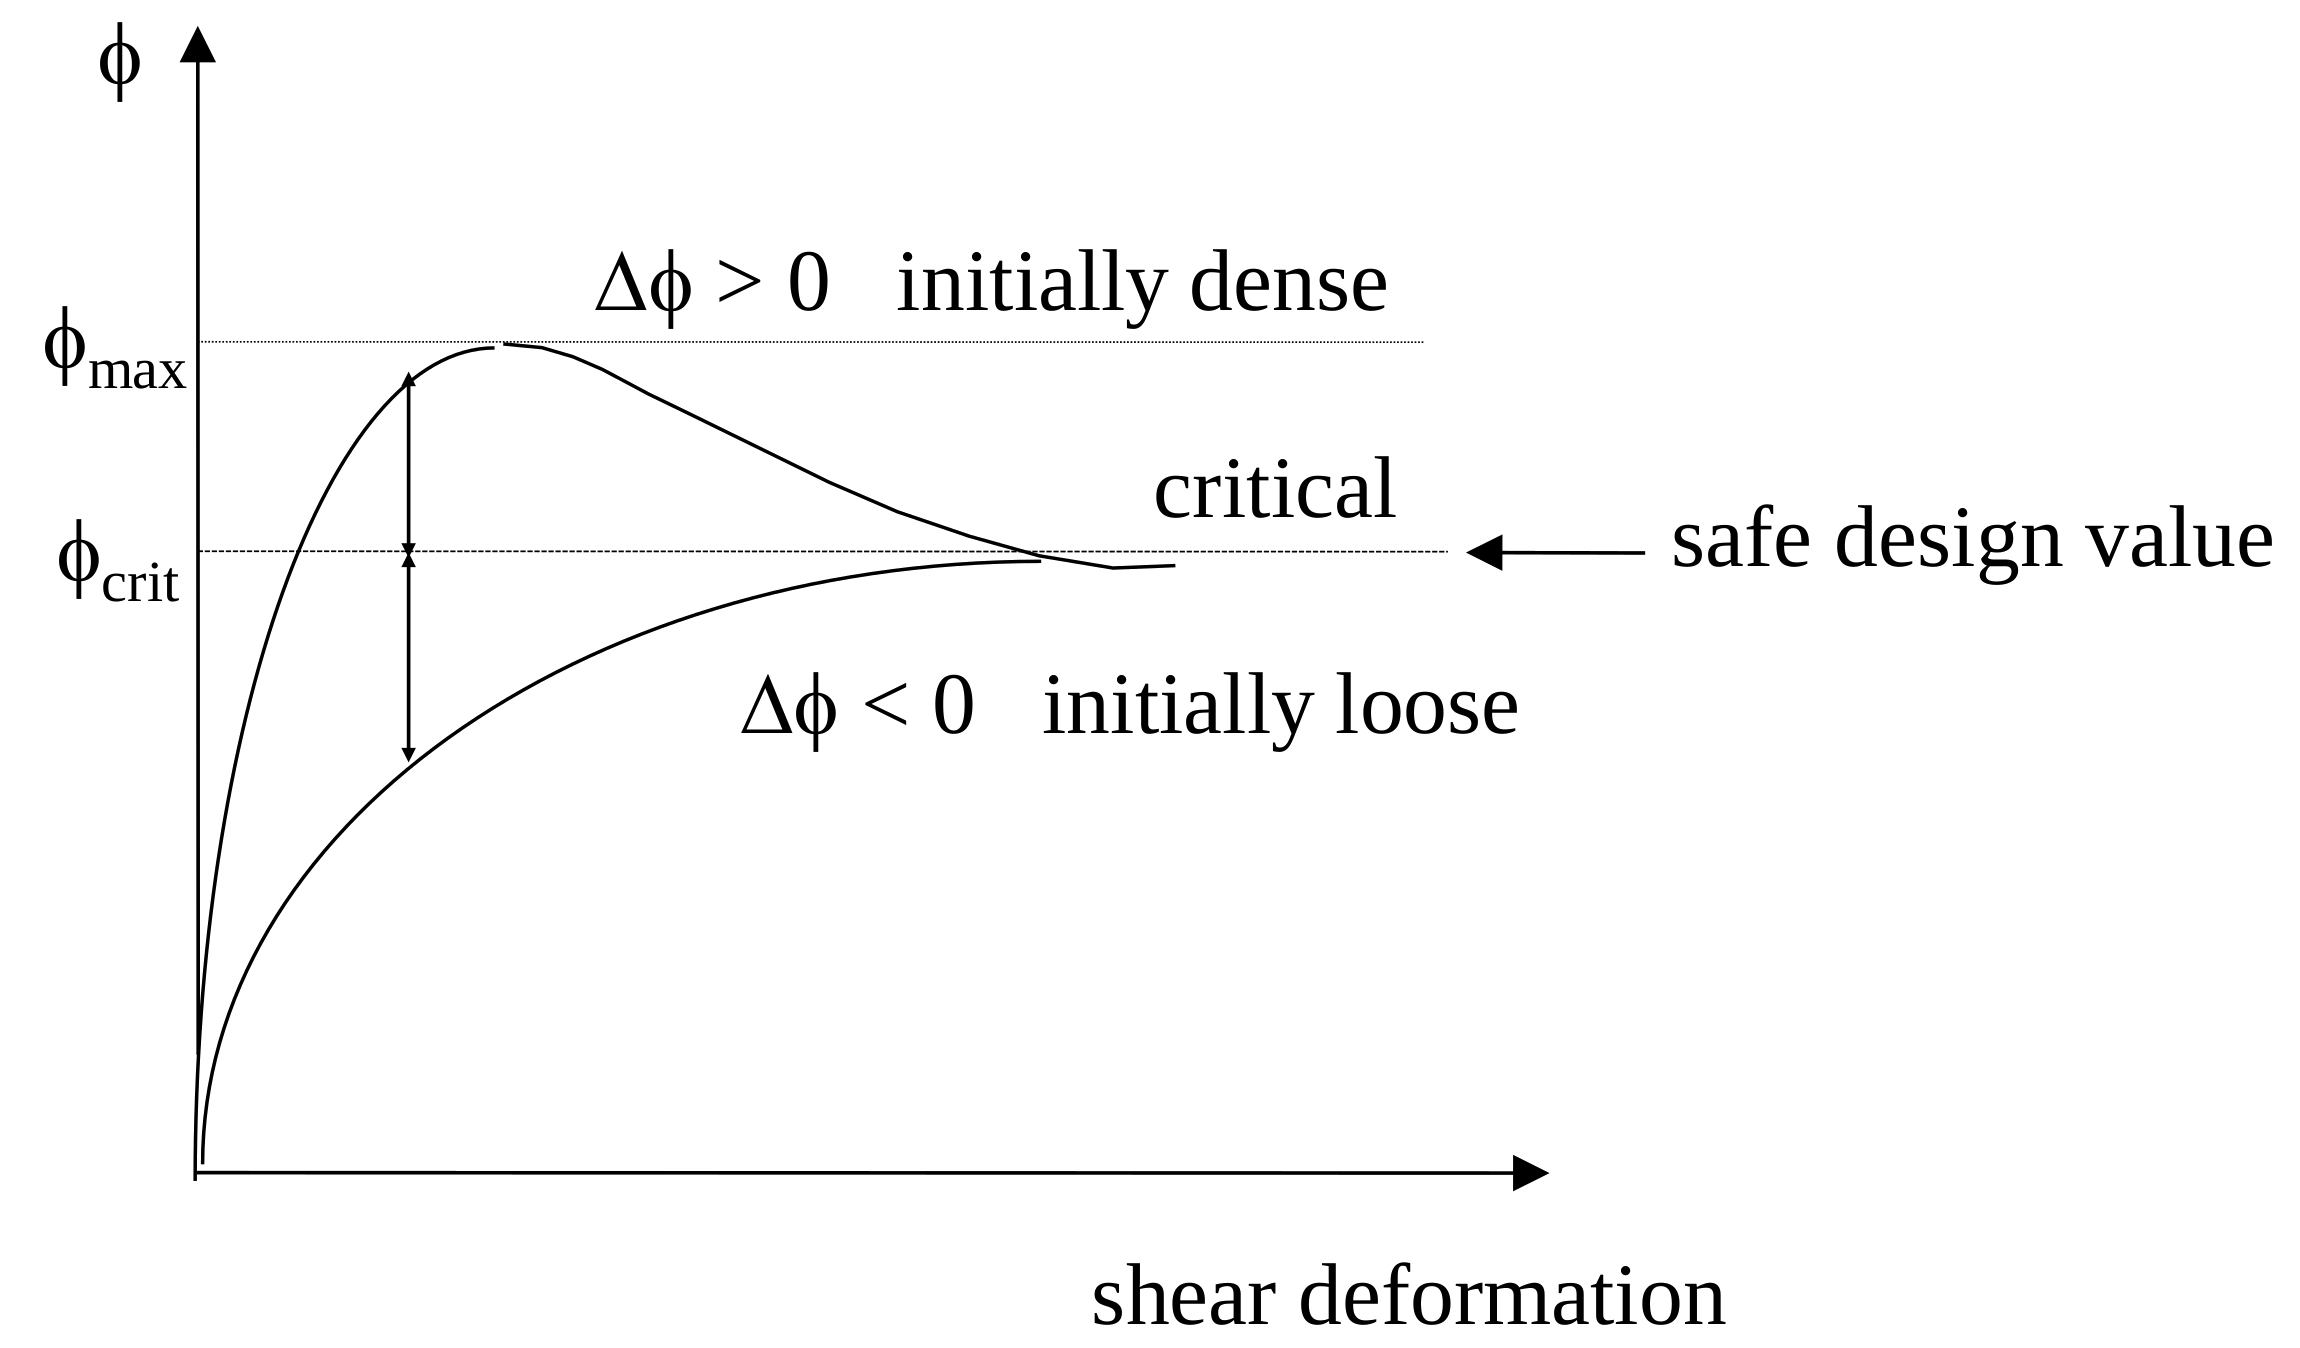
\includegraphics[width=\textwidth]{figs/macroscopic-friction.png}
	\end{figure}
	\mode<beamer>{	
		\begin{equation*}
		\phi = \phi_{cs} + \Delta \phi_{dilatancy}
		\end{equation*}
	}
	\mode<handout>{
		\vspace{6cm}
	}
\end{frame}


%----------------------------------------------------------------------------------------
\begin{frame}
	\frametitle{Critical state friction angle and density}
	\begin{figure}
		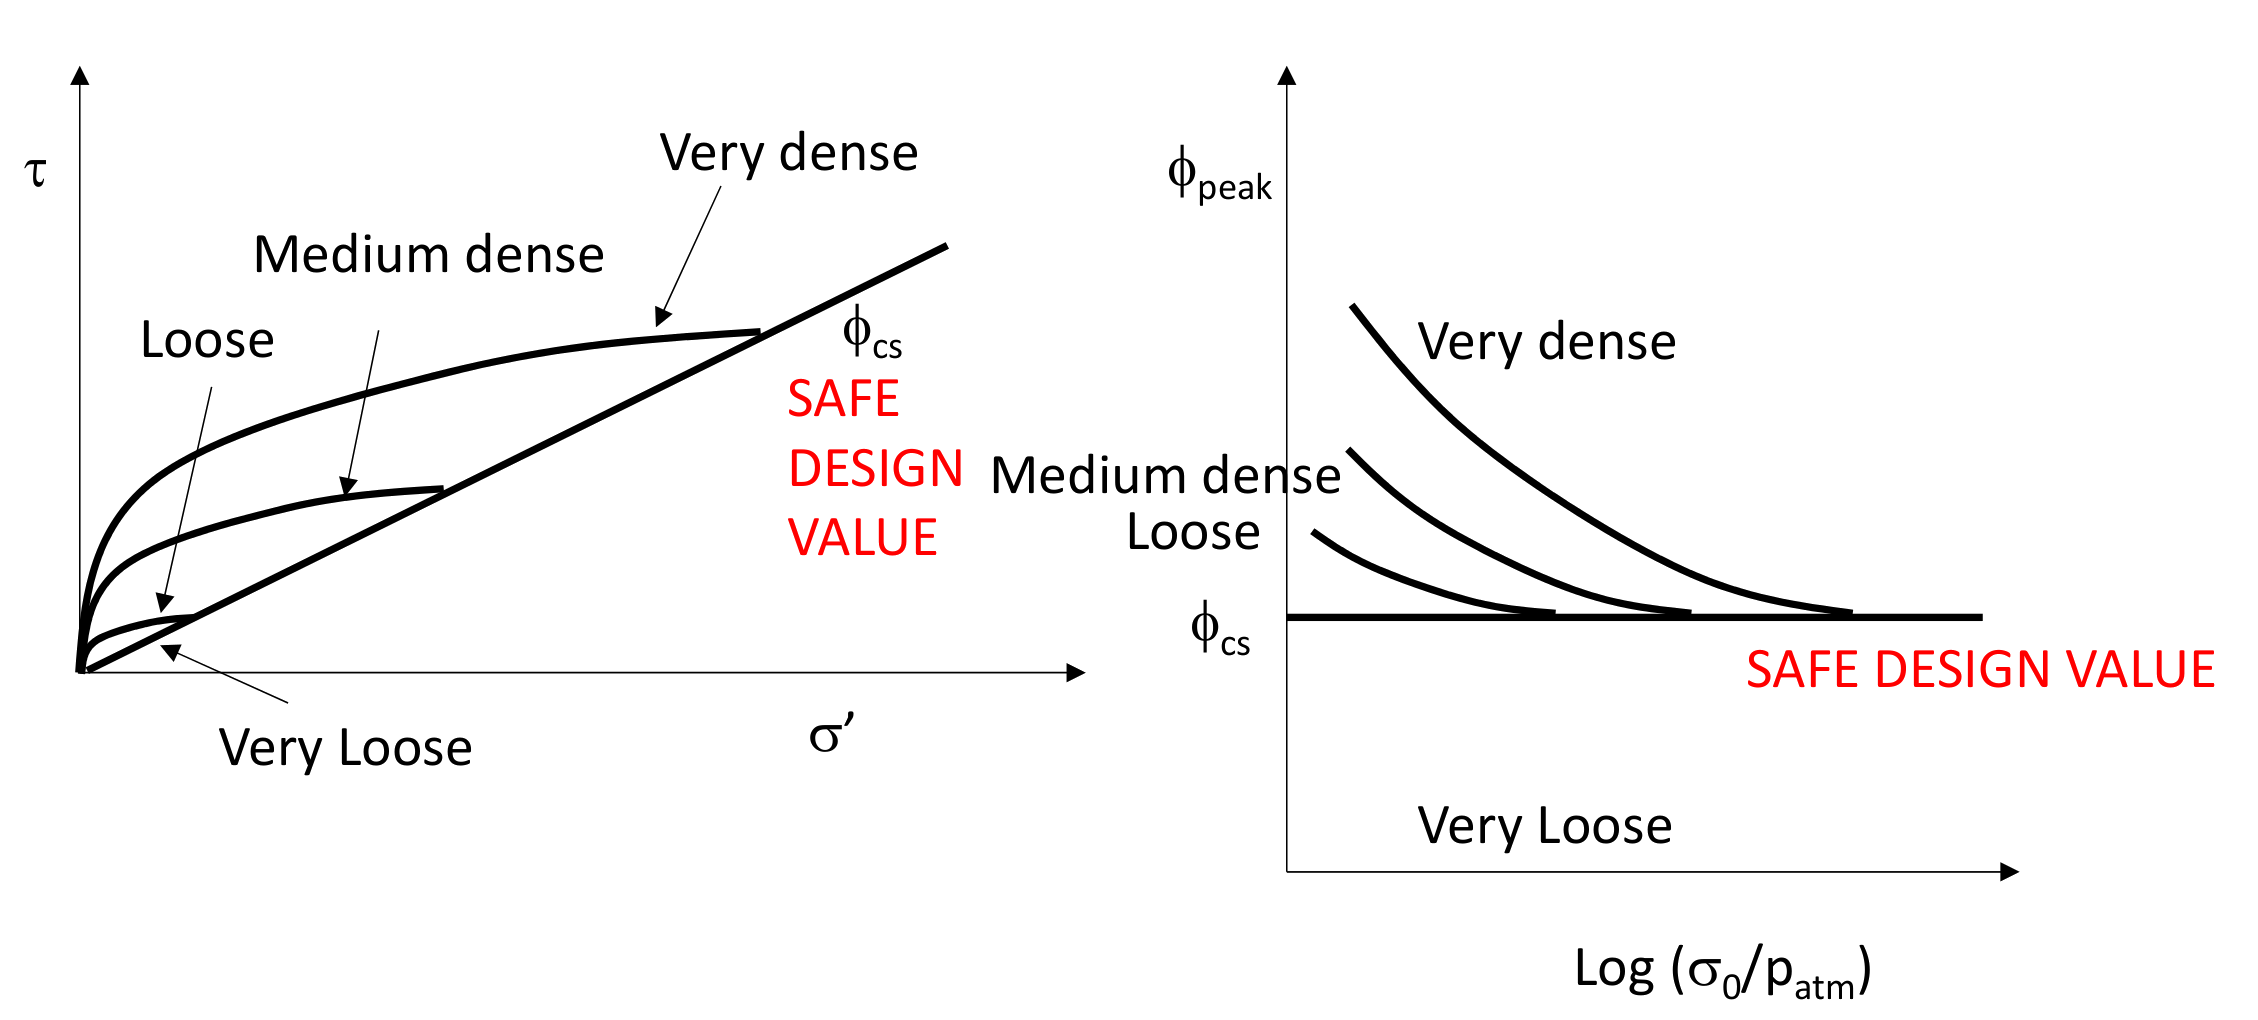
\includegraphics[width=0.95\textwidth]{figs/sand-friction-angle.png}
	\end{figure}
	\mode<beamer>{
		\begin{equation*}
		\phi_{peak} = \phi_{cs} + \Delta \phi (\text{confining stress, initial void ratio})
		\end{equation*}
	}
	\mode<handout>{
		\vspace{2cm}
	}
\end{frame}


%----------------------------------------------------------------------------------------
\begin{frame}
	\frametitle{Dilation angle $\psi$}
	\begin{figure}
		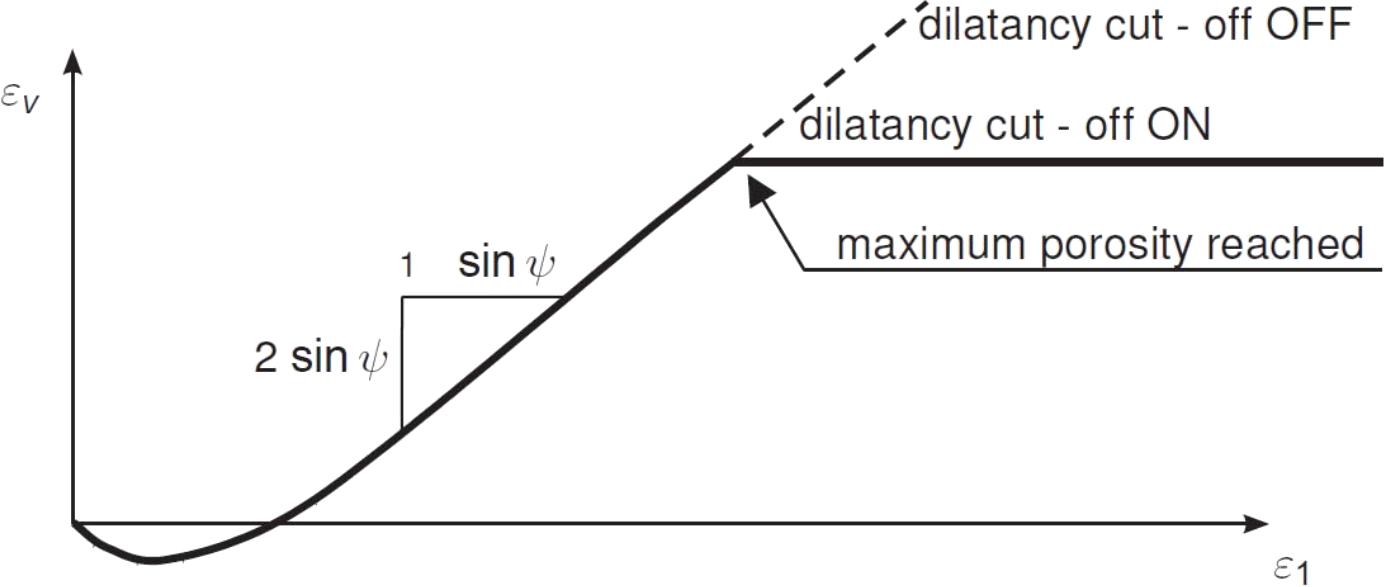
\includegraphics[width=0.95\textwidth]{figs/sand-dilation.png}
	\end{figure}
	\mode<beamer>{
		\begin{enumerate}
			\item Simulate CD or CU test and check the volume change behavior (for
			CD) and excess pore pressure behavior (for CU)!
			\item For CU, if the computed undrained shear strength is greater than the
			actual value, use Undrained (B).
		\end{enumerate}
	}
	\mode<handout>{
		\vspace{2cm}
	}
\end{frame}

%----------------------------------------------------------------------------------------
\begin{frame}
	\frametitle{Friction angle (Bolton., 1986)}
	Friction angle
	\mode<beamer>{
		\begin{align*}
		\phi_{peak} - \phi_{cs} & = 3I_R \quad \text{for triaxial compression} \\
		& = 5 I_R \quad \text{for plane strain}
		\end{align*}
		Relative density index
		\begin{align*}
		I_R & = I_D \cdot I_c - 1 \\
		\text{Relative crushability } I_c & =  \ln \left(\frac{\sigma_c}{p^\prime}\right)\\
		\sigma_c \text{ for quartz} & = 20 GPa \\
		\text{Relative density } I_D & = \frac{e_{max} - e}{e_{max} - e_{min}}
		\end{align*}
		Dilation angle
		\begin{align*}
		\psi & \approx 1.25 (\phi_{peak} - \phi_{cs})\\
		\psi & = 0 \text{ when } \phi_{peak} = \phi_{cs}
		\end{align*}
	}
	\mode<handout>{
		\vspace{2cm}
	}
\end{frame}

%----------------------------------------------------------------------------------------
\begin{frame}
	\frametitle{Macroscopic friction angle}
	\begin{itemize}
		\item $\phi_{crit}$ is the angle of friction measured at constant volume of a soil
		aggregate, and $\Delta \phi$ dilatancy is the extra dilatant contribution to
		friction angle $\phi$. Typical values are:
		\item Critical state friction $\phi_{crit}$:
		\begin{itemize}
			\item clay: $\ang{22}$
			\item uniform rounded sand: $\ang{32}$
			\item well-graded angular sandy gravel: $\ang{38}$
		\end{itemize}
		\item peak strength of pre-compressed or uncrushable grains, densely compacted, and:
		shearing in plane strain $\Delta \phi$:
		\begin{itemize}
			\item shearing in plane strain: $\Delta \phi_{max} = \ang{20}$
			\item shearing in axial symmetry: $\Delta \phi_{max} = \ang{12}$
		\end{itemize}
	\end{itemize}
\end{frame}


%----------------------------------------------------------------------------------------
\begin{frame}
	\frametitle{Discrete Element Method}
	\noindent
	\fboxsep=0pt
	\noindent
	\begin{minipage}[t]{0.65\linewidth}
		\begin{enumerate}
			\item Particle level interaction based on
			Newton's equation of motion
			\item The contact normal force is
			computed as:
			\begin{equation*}
			F_n = %
			\begin{cases}
			0, \quad \delta_n > 0\\
			-k_n \delta_n - \gamma_n \frac{d \delta_n}{dt}, \quad \delta_n < 0
			\end{cases}
			\end{equation*}
			\item The contact tangential force is
			computed in a similar way, but
			has a frictional limit.
			\begin{equation*}
			F_t \le \mu F_n
			\end{equation*}
			\item Solve Newton's second law and
			the angular momentum equation
			(including rotational resistance).
		\end{enumerate}
		
	\end{minipage}%
	\hfill
	\begin{minipage}[t]{0.35\linewidth}
		\begin{figure}
			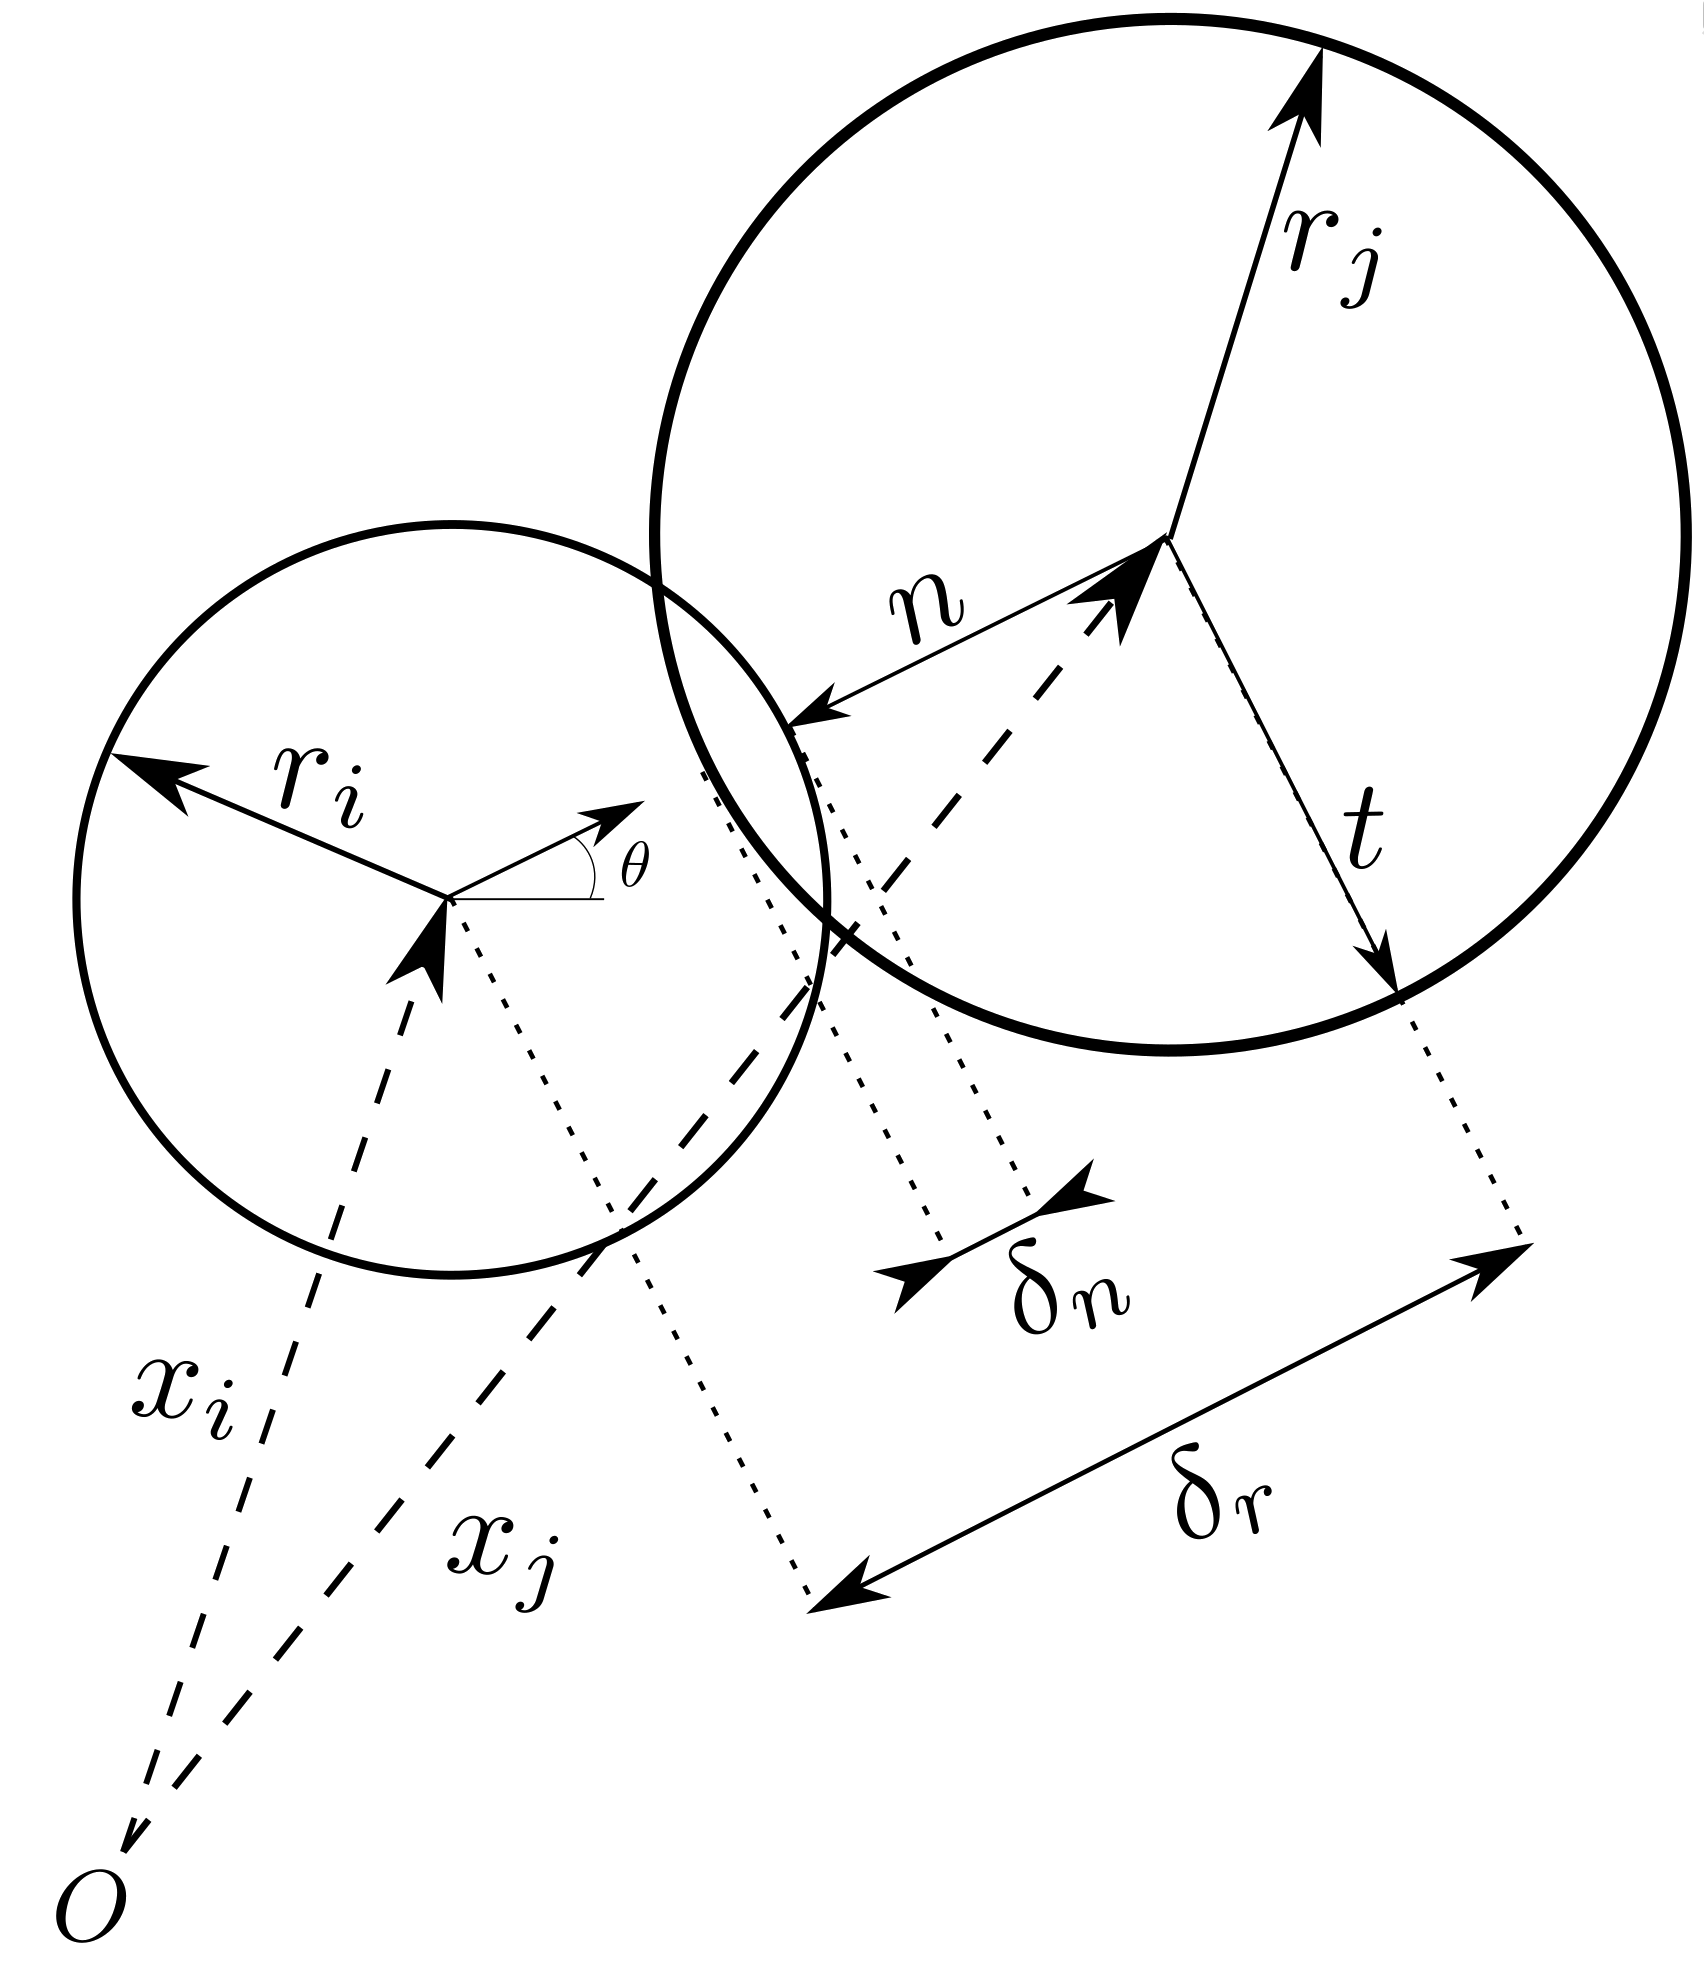
\includegraphics[width=\textwidth]{figs/dem.png}
		\end{figure}
	\end{minipage}	
\end{frame}

%----------------------------------------------------------------------------------------
\begin{frame}
	\frametitle{Strong force network vs weak clusters}
	\begin{figure}
		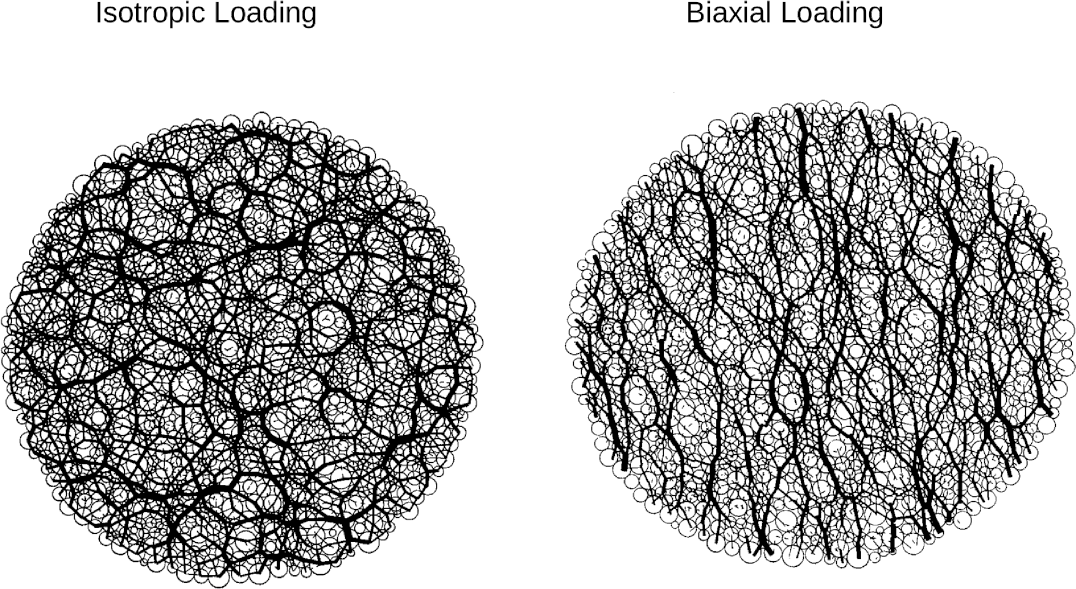
\includegraphics[width=\textwidth]{figs/force-network-weak-clusters.png}
	\end{figure}
\end{frame}

%----------------------------------------------------------------------------------------
\begin{frame}
	\frametitle{Fabric anisotropy}
	\begin{figure}
		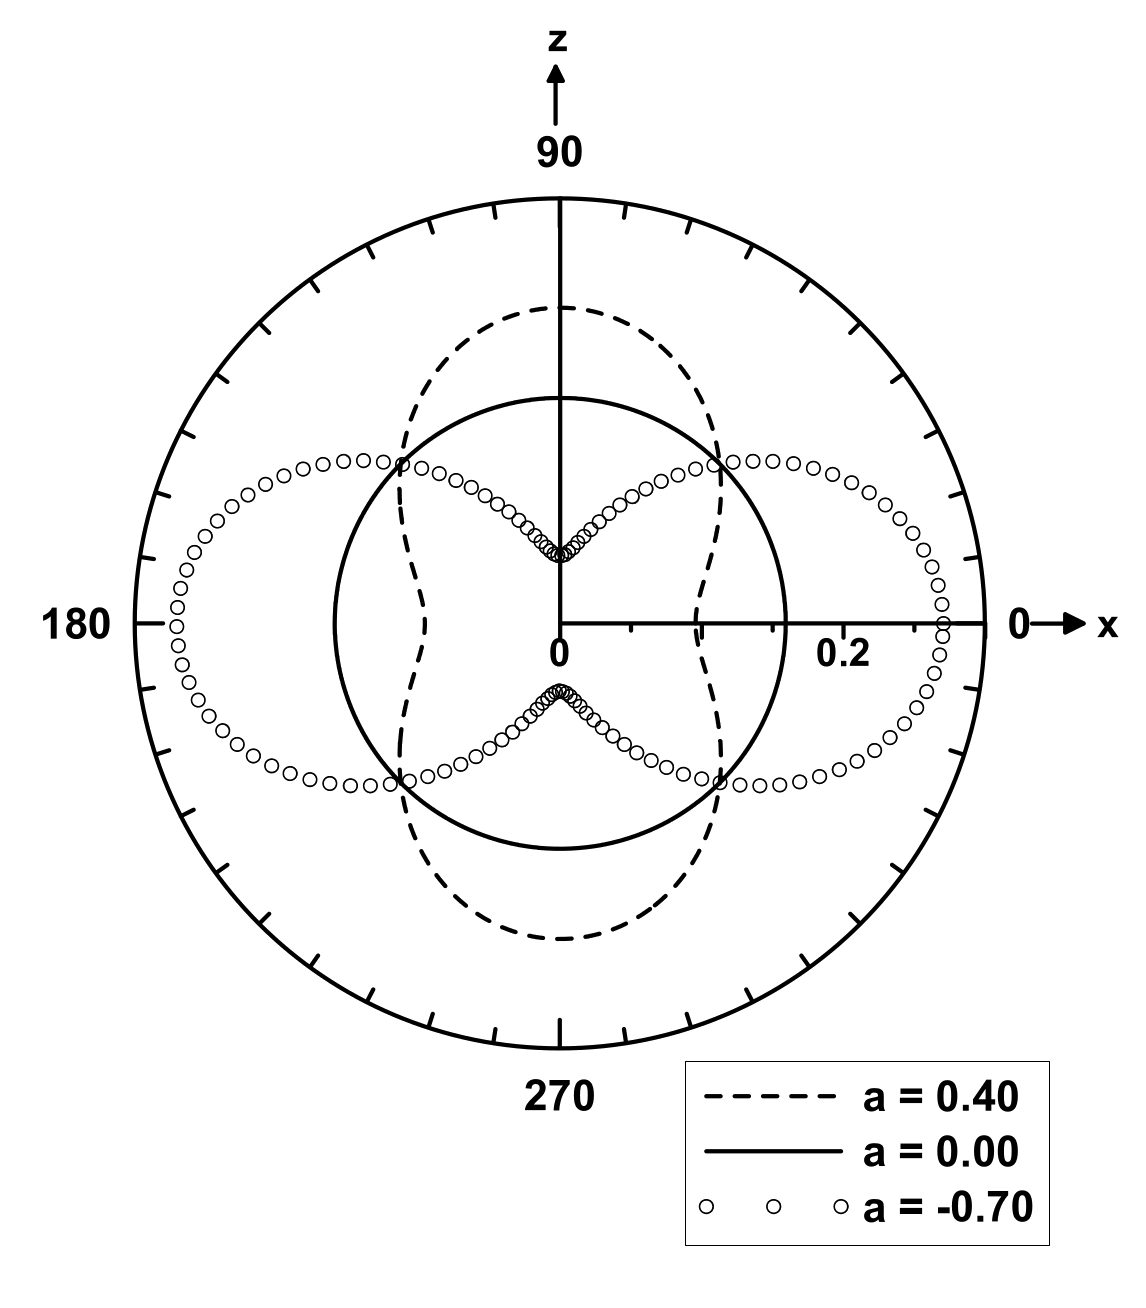
\includegraphics[width=0.5\textwidth]{figs/fabric-anisotropy.png}
		\caption*{Fabric anisotropy under different stress conditions}
	\end{figure}
\end{frame}


%----------------------------------------------------------------------------------------
\begin{frame}
	\frametitle{Interparticle friction angles}
	\begin{itemize}
		\item For Quartz Sands: 26 degrees
		\item  For Sheet Minerals (muscovite, phlogopite, biotite and chlorite): 7 - 13 degrees
		\begin{itemize}
			\item Water acts as a lubricant
		\end{itemize}
		\item Clay minerals: Probably 7 - 13 degrees
		\begin{itemize}
			\item Similar to reported residual friction angles.
			\item Sodium Montmorillonite: 4 degrees
		\end{itemize}
	\end{itemize}
\end{frame}

%----------------------------------------------------------------------------------------
\begin{frame}
	\frametitle{Micro to Macroscopic friction angle}
	\begin{figure}
		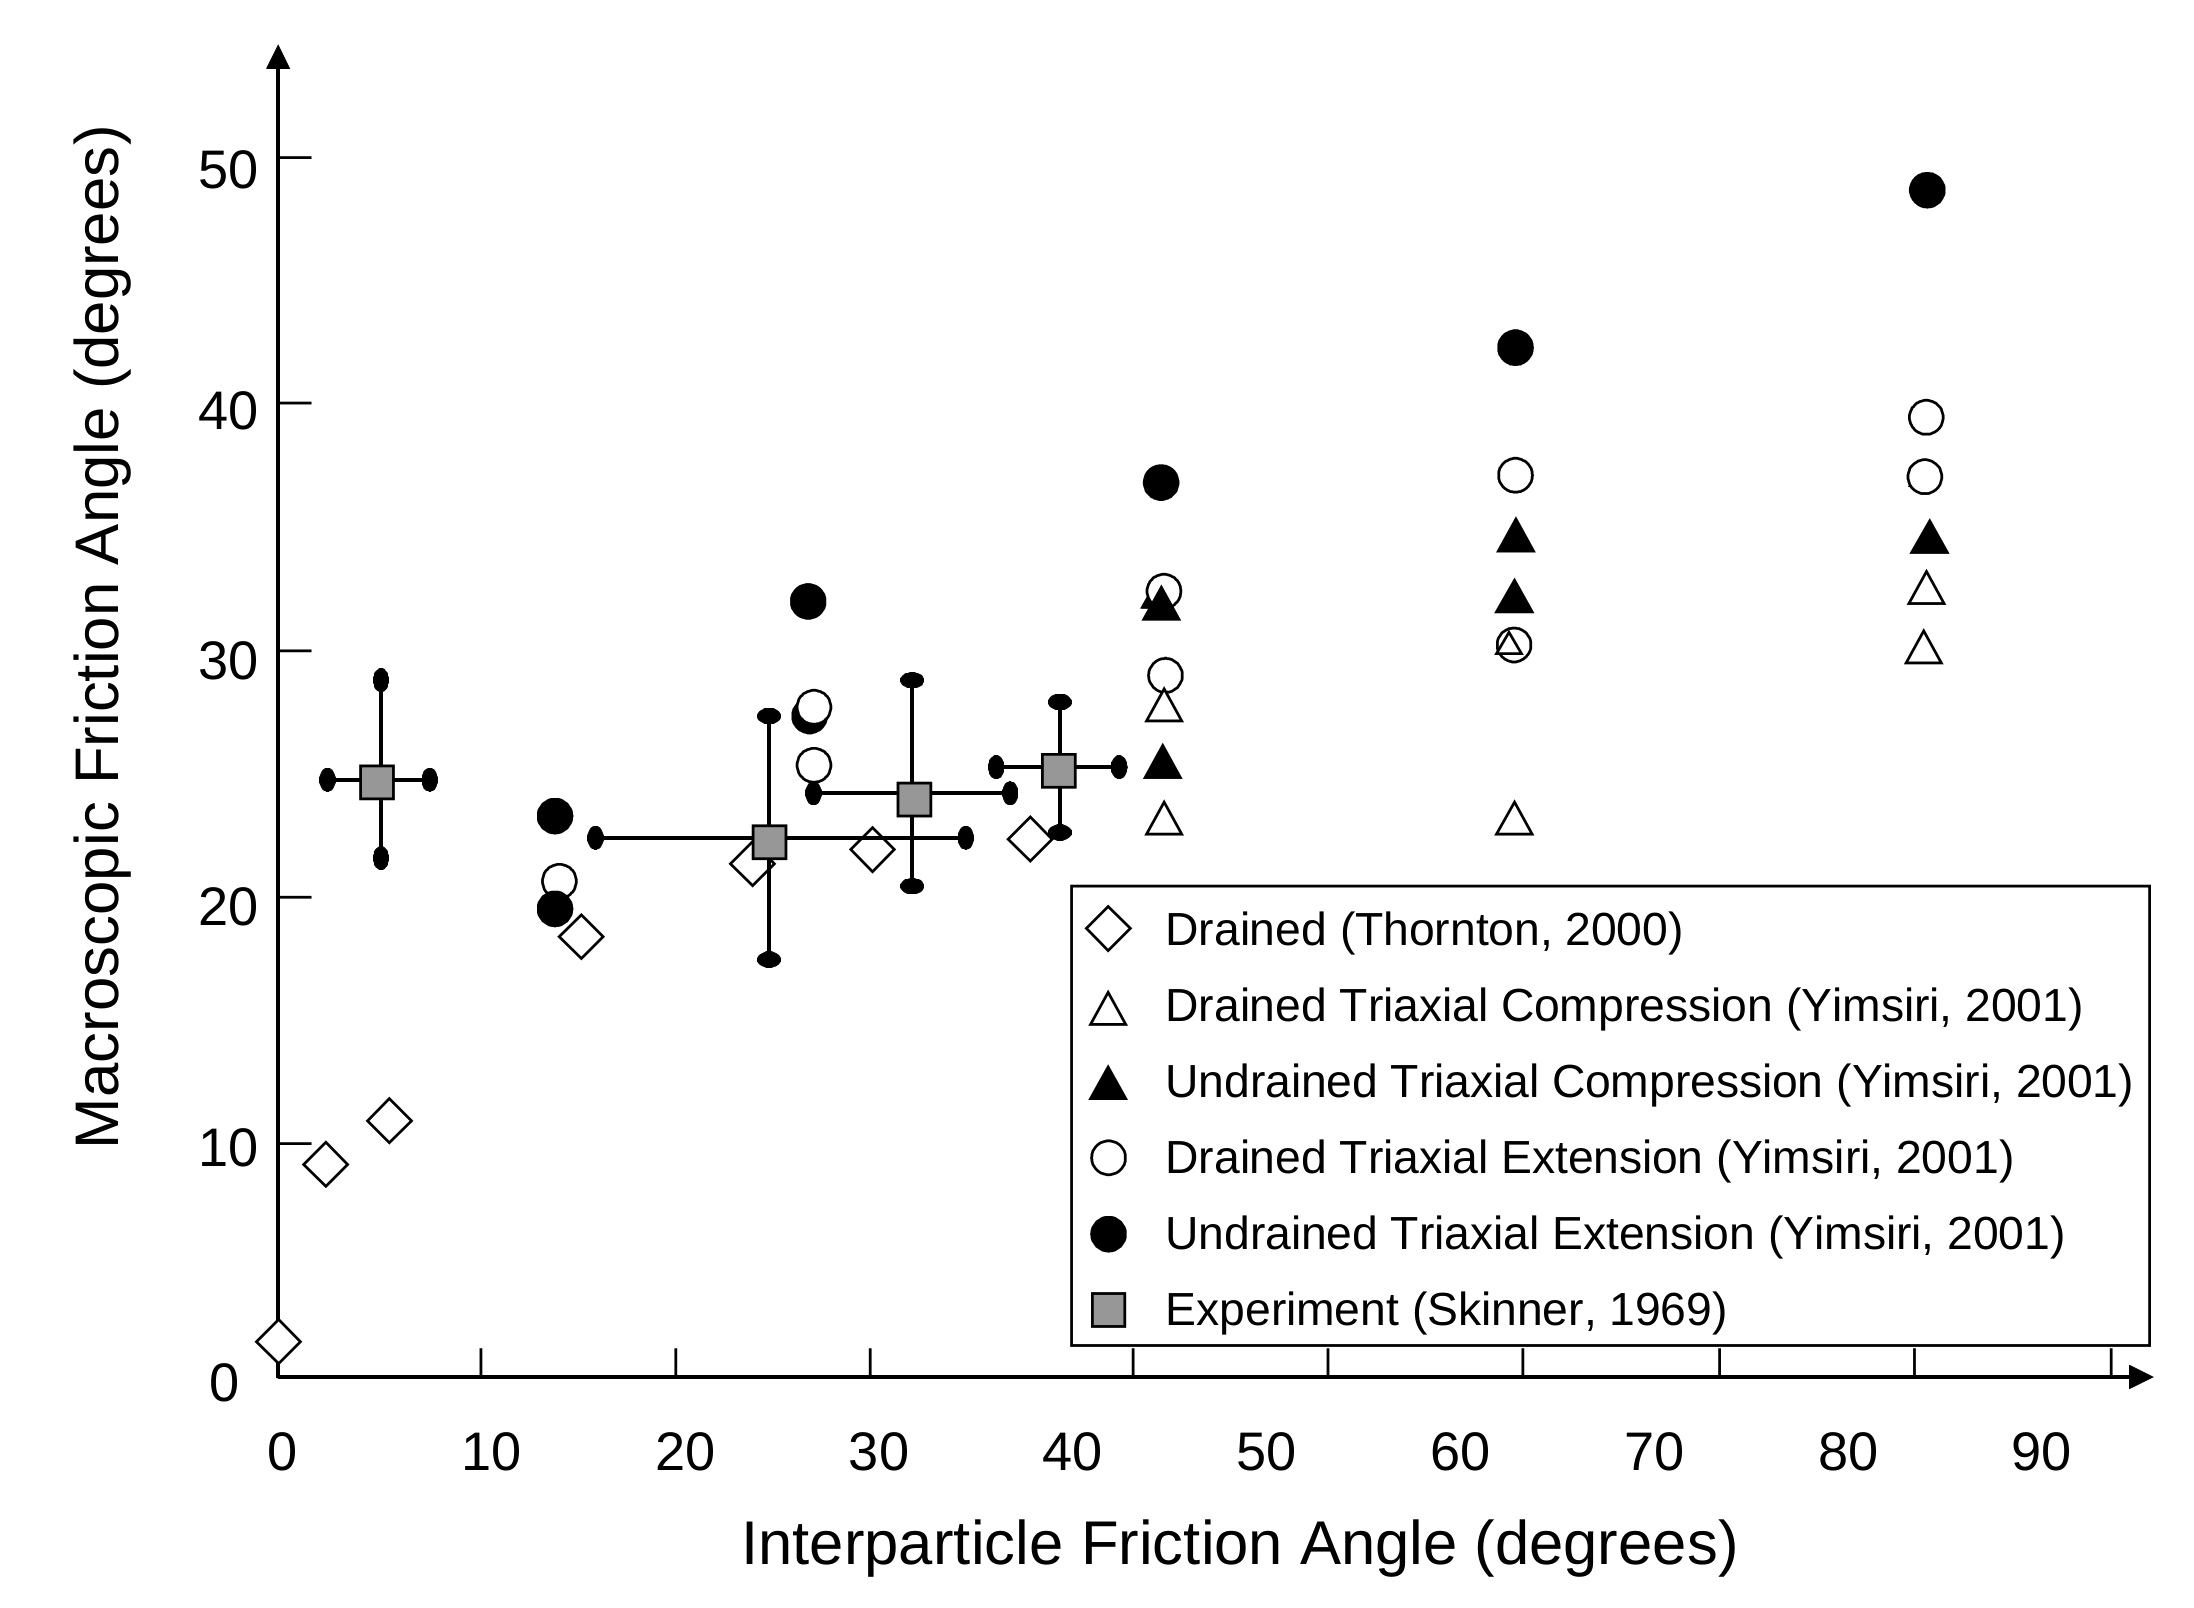
\includegraphics[width=0.75\textwidth]{figs/macroscopic-interparticle-friction.png}
		\caption*{Relationship between macroscopic friction angle and interparticle friction angle (no rolling resistance) - Yimisir and Soga (2001)}
	\end{figure}
\end{frame}


%----------------------------------------------------------------------------------------
\begin{frame}
	\frametitle{Micro to Macroscopic friction angle: Rolling resistance}
	\begin{figure}
		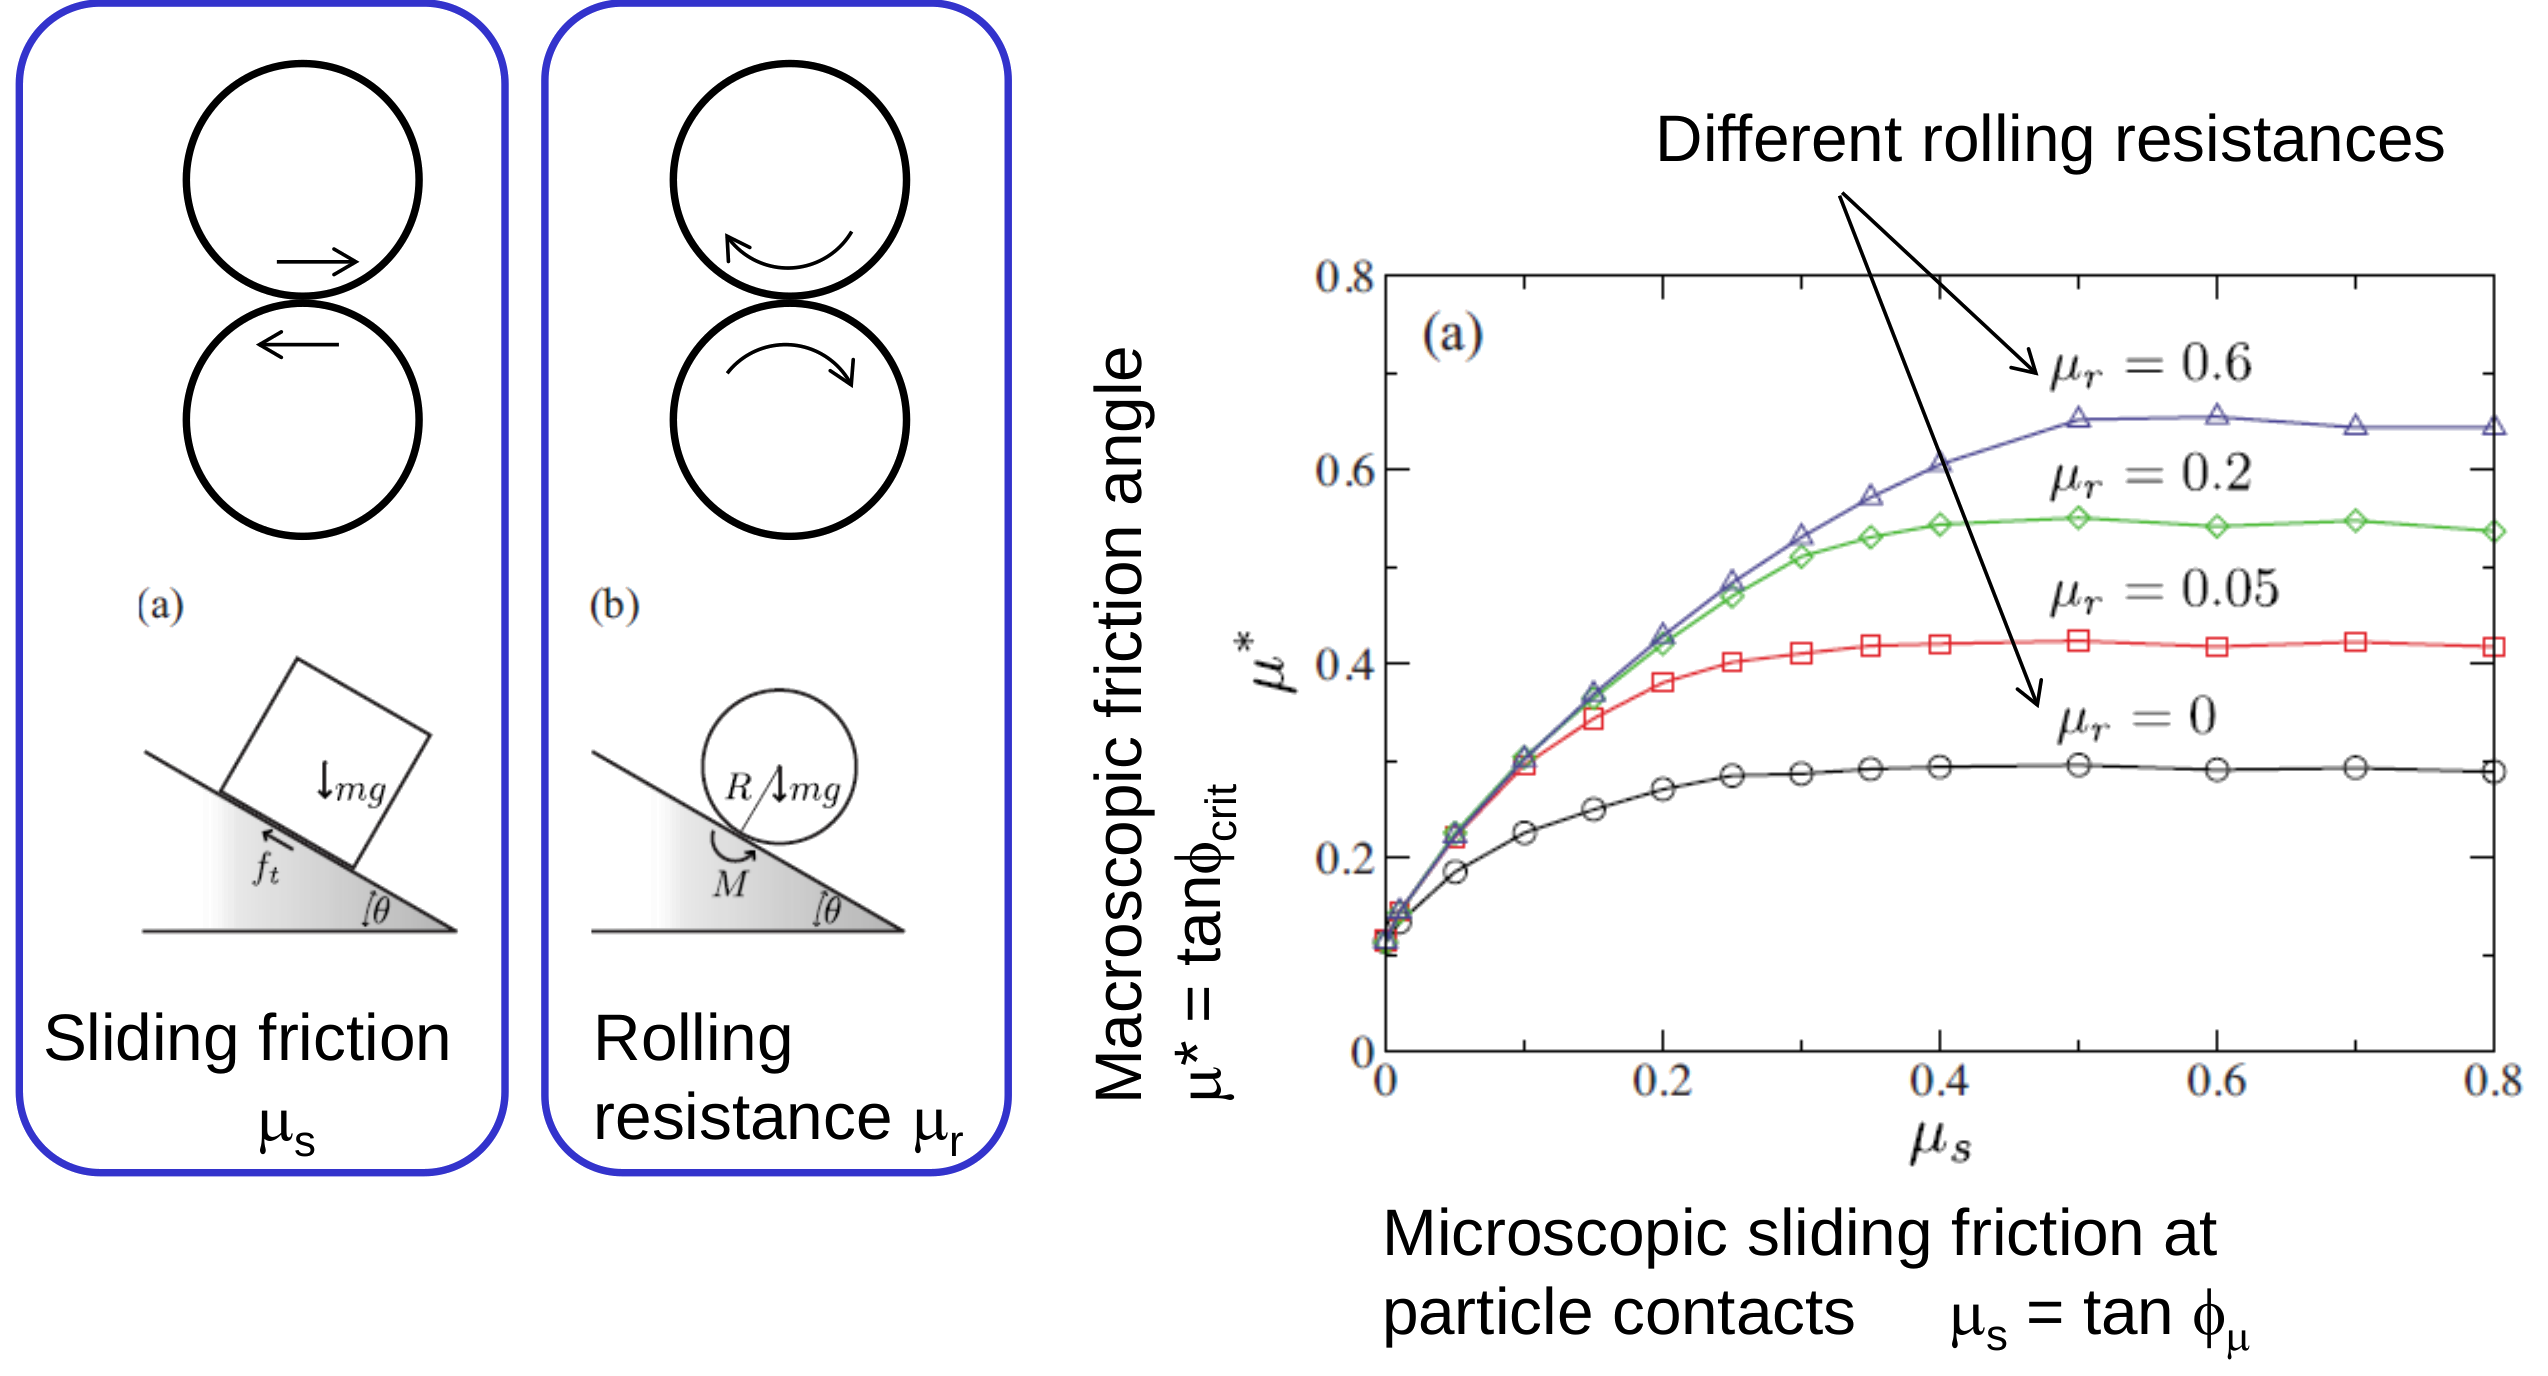
\includegraphics[width=\textwidth]{figs/rolling-resistance.png}
		\caption*{Estrada et al., (2001)}
	\end{figure}
\end{frame}

%----------------------------------------------------------------------------------------
\begin{frame}
	\frametitle{Interparticle friction angles}
	\noindent
	\fboxsep=0pt
	\noindent
	\begin{minipage}[t]{0.65\linewidth}
		\begin{itemize}
			\item The interparticle friction acts as a kinematic
			constraint of the strong force network and not as
			the direct source of macroscopic resistance to
			shear.
			\item Increased friction at the contacts increases the
			stability of the system (development of
			anisotropic fabric) and reduces the number of
			contacts required to achieve a stable condition.
			\item As long as the strong force network can be
			formed, the magnitude of the interparticle friction
			becomes of secondary importance.
		\end{itemize}
	\end{minipage}%
	\hfill
	\begin{minipage}[t]{0.35\linewidth}
		\begin{figure}
			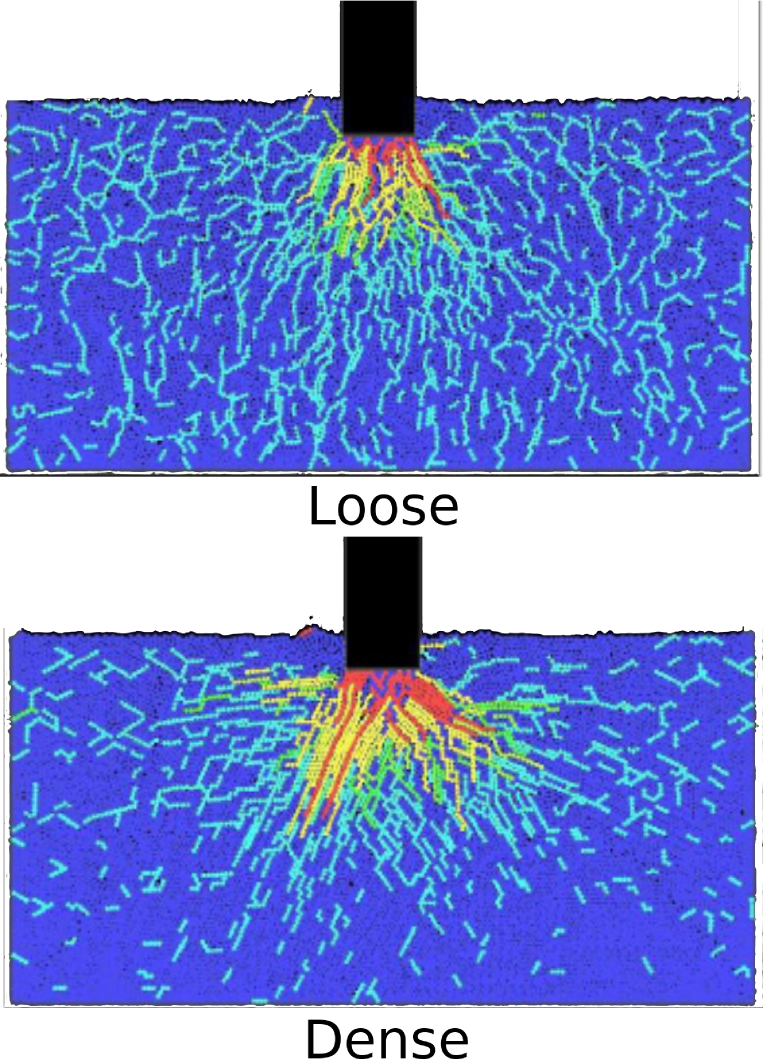
\includegraphics[width=\textwidth]{figs/dem-force-chains-punch.png}
			\caption*{Muthuswamy and Tordesillas (2006)}
		\end{figure}
	\end{minipage}
\end{frame}

%----------------------------------------------------------------------------------------
\begin{frame}
	\frametitle{What is dilation? shear band}
	\begin{figure}
		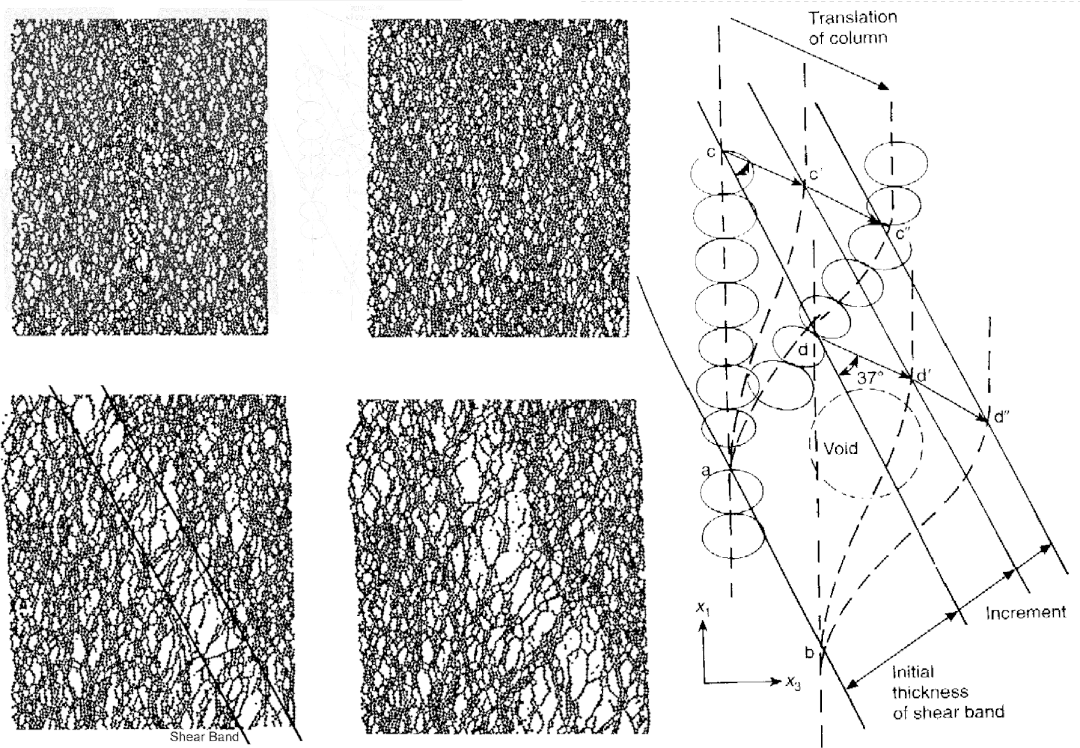
\includegraphics[width=0.85\textwidth]{figs/dilation.png}
		\caption*{Iwashita and Oda (2000)}
	\end{figure}
\end{frame}

\note{Kuhn (1999) reports that their thicknesses
	are $1.5 D_{50}$ to $2.5D_{50}$ in the early stages of shearing and increase to between $1.5D_{50}$ and $4D_{50}$ as deformation
	proceeds.}

%----------------------------------------------------------------------------------------
\begin{frame}
	\frametitle{Fabric evolution at critical state}
	\begin{figure}
		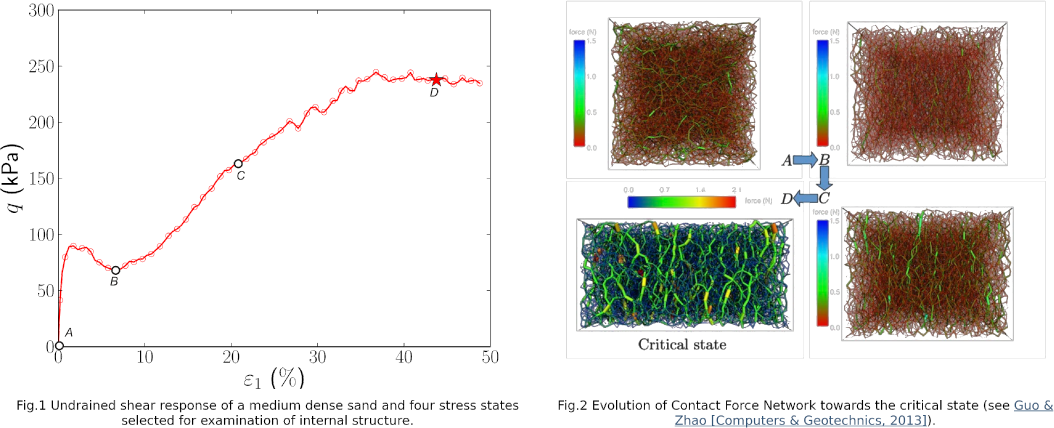
\includegraphics[width=\textwidth]{figs/fabric-evolution-cs.png}
		\caption*{Guo and Zhao (2003)}
	\end{figure}
\end{frame}


\note{
	As deformation progresses,
	\begin{itemize}
		\item The number of particles in the strong force network decreases.
		\item With fewer particles sharing the increased loads.
		\item Anisotropic fabric develops, showing the formation of strong force network. Fabric of particles associated with strong forces is different from that associated with weak
		clusters.
		\item At critical state, force chain forms and buckles continuously. Likely to buckle when a force chain has 8 	particles
	\end{itemize}
}

\end{document}
